%--------------------------------------------------------------
% thesis.tex 
%--------------------------------------------------------------
% Corso di Laurea in Informatica 
% http://if.dsi.unifi.it/
% @Facolt\`a di Scienze Matematiche, Fisiche e Naturali
% @Universit\`a degli Studi di Firenze
%--------------------------------------------------------------
% - template for the main file of Informatica@Unifi Thesis 
% - based on Classic Thesis Style Copyright (C) 2008 
%   Andr\'e Miede http://www.miede.de   
%--------------------------------------------------------------
\documentclass[twoside,openright,titlepage,fleqn,
	headinclude,12pt,a4paper,BCOR5mm,footinclude]{scrbook}
%--------------------------------------------------------------
\newcommand{\myItalianTitle}{Sviluppo di un'applicazione Android per il posizionamento indoor\xspace}
\newcommand{\myEnglishTitle}{Developement of an indoor positioning Android application\xspace}
% use the right myDegree option
\newcommand{\myDegree}{Corso di Laurea in Informatica\xspace}
%\newcommand{\myDegree}{
	%Corso di Laurea Specialistica in Scienze e Tecnologie 
	%dell'Informazione\xspace}
\newcommand{\myName}{Michele De Vita\xspace}
\newcommand{\myProf}{Andrea Ceccarelli\xspace}
\newcommand{\myOtherProf}{\xspace}
\newcommand{\mySupervisor}{Nome Cognome\xspace}
\newcommand{\myFaculty}{
	Scuola di Scienze Matematiche, Fisiche e Naturali\xspace}
\newcommand{\myUni}{\protect{
	Universit\`a degli Studi di Firenze}\xspace}
\newcommand{\myLocation}{Firenze\xspace}
\newcommand{\myTime}{Anno Accademico 2014-2015\xspace}
\newcommand{\myVersion}{Version 0.1\xspace}


%--------------------------------------------------------------

\usepackage[italian]{babel}
\usepackage[latin1]{inputenc} 
\usepackage[T1]{fontenc} 
\usepackage[square,numbers]{natbib} 
\usepackage[fleqn]{amsmath}  
\usepackage{ellipsis}
\usepackage{listings}
\usepackage{subfig}  
\usepackage{caption} 
\usepackage{appendix}
\usepackage{siunitx} 
\usepackage{float}   
\usepackage[colorlinks=true, linkcolor=black, urlcolor=blue]{hyperref}


%--------------------------------------------------------------
\usepackage{dia-classicthesis-ldpkg}
%--------------------------------------------------------------
% Options for classicthesis.sty:
% tocaligned eulerchapternumbers drafting linedheaders 
% listsseparated subfig nochapters beramono eulermath parts 
% minionpro pdfspacing
\usepackage[eulerchapternumbers,linedheaders,subfig,beramono,eulermath,
parts]{classicthesis}
%--------------------------------------------------------------
\newlength{\abcd} % for ab..z string length calculation
% how all the floats will be aligned
\newcommand{\myfloatalign}{\centering} 
\setlength{\extrarowheight}{3pt} % increase table row height
\captionsetup{format=hang,font=small}
\setcounter{secnumdepth}{3}
%--------------------------------------------------------------
% Layout setting
%--------------------------------------------------------------
\usepackage{geometry}
\geometry{
	a4paper,
	ignoremp,
	bindingoffset = 1cm, 
	textwidth     = 13.5cm,
	textheight    = 21.5cm,
	lmargin       = 3.5cm, % left margin
	tmargin       = 4cm    % top margin 
}

\lstset{
  	frame=tb,
	language=Matlab,
  	aboveskip=3mm,
  	belowskip=3mm,
  	showstringspaces=false,
  	columns=flexible,
  	basicstyle={\small\ttfamily},
  	numbers=none,
  	breaklines=true,
  	breakatwhitespace=true,
  	tabsize=3
}
%--------------------------------------------------------------
\begin{document}
\frenchspacing
\raggedbottom
\pagenumbering{roman}
\pagestyle{plain}
%--------------------------------------------------------------
% Frontmatter
%--------------------------------------------------------------
%--------------------------------------------------------------
% titlepage.tex (use thesis.tex as main file)
%--------------------------------------------------------------
\begin{titlepage}
	\begin{center}
   	\large
      \hfill
      \vfill
      \begingroup
         
\includegraphics[scale=0.15]{logo/LOGO}\\
%			\spacedallcaps{\myUni} \\ 
			\myFaculty \\
			\myDegree \\ 
			\vspace{0.5cm}
         \vspace{0.5cm}    
         Tesi di Laurea    
      \endgroup 
      \vfill 
      \begingroup
      	\color{Maroon}\spacedallcaps{\myItalianTitle} \\ $\ $\\
      	\spacedallcaps{\myEnglishTitle} \\ 	
	\bigskip
      \endgroup
      \spacedlowsmallcaps{\myName}
      \vfill 
      \vfill
      Relatore: \emph{Relatore}\\
      Correlatore: \emph{Correlatore}\\
      \vfill
      \vfill
      \myTime
      \vfill                      
	\end{center}        
\end{titlepage}   
%--------------------------------------------------------------
% back titlepage
%--------------------------------------------------------------
   \newpage
	\thispagestyle{empty}
	\hfill
	\vfill
	\noindent\myName: 
	\textit{\myItalianTitle,} 
	\myDegree, \textcopyright\ \myTime
%--------------------------------------------------------------
% back titlepage end
%--------------------------------------------------------------
\pagestyle{scrheadings}
%--------------------------------------------------------------
% Mainmatter
%--------------------------------------------------------------
\pagenumbering{arabic}
% use \cleardoublepage here to avoid problems with pdfbookmark
%\include{intro} % use \myChapter command instead of \chapter
\tableofcontents
\listoffigures
\cleardoublepage
\thispagestyle{empty}
\begin{flushright}
\null\vspace{\stretch {1}}
\emph{"Inserire citazione" \break --- Inserire autore citazione} \vspace{\stretch{2}}\null
\end{flushright}
\cleardoublepage

\chapter{Introduzione}
La seguente tesi \`e basata su un tirocinio esterno svolto con l'azienda $KeepUp$ in cui \`e stata sviluppata la base di un'applicazione Android col compito di localizzare all'interno degli edifici la posizione dello \textit{smartphone} sfruttando le distorsioni del campo magnetico terrestre\cite{6418880}.
\\\\
Un'applicazione del genere ha molti usi in luoghi chiusi aperti al pubblico: per esempio immaginiamoci di trovarci in un museo. In questo caso l'applicazione ufficiale del museo che supporta l'\textit{indoor positioning} ci localizza all'interno di una mappa $2D$ dell'edificio perci\`o riesce a capire se ci avviciniamo ad un'opera d'arte e quando avviene, si apre un \textit{pop-up} che ci fornisce informazioni aggiuntive su ci\`o che stiamo osservando. Oppure immaginiamoci di dover prendere l'aereo e di essere in ritardo in un aeroporto all'estero che non conosciamo affatto. Un navigatore \textit{indoor} potrebbe far molto comodo a chi si trova in questa situazione perch\'e gli permetterebbe di raggiungere il proprio \textit{gate} in pochissimo tempo senza conoscere la piantina dell'aeroporto.
\\\\
Il primo capitolo \`e questo, una semplice introduzione al lavoro svolto.
\\\\
Durante il secondo capitolo, i fondamentali, approfondiremo il tipo di dato che dobbiamo trattare, le sue origini e la sua struttura per poi passare all'apprendimento automatico, usato per predire la posizione dell'utente all'interno dell'edificio elencandone i vari tipi e definendo alcuni termini gergali per concludere con la descrizione approfondita di alcuni classificatori molto conosciuti nel mondo dell'AI.
\\\\
Nel terzo capitolo parleremo della struttura del software \textit{Android} realizzato durante il tirocinio, dai linguaggi e librerie usate alla struttura del codice implementato.
\\\\
Nel quarto capitolo vedremo i risultati ottenuti dai dati estratti della nostra applicazione tramite vari grafici che mostrano i vari punti di forza e debolezza.
\\\\
Nel quinto capitolo trattiamo dei possibili miglioramenti futuri all'applicazione e delle conclusioni.
\chapter{Fondamentali}
L'identificazione della posizione all'interno di un edificio si svolge in 3 fasi:
\begin{enumerate}
	\item Scansione dell'ambiente
	\item Costruzione di un modello
	\item Ricerca della posizione
\end{enumerate}

Nelle successive 3 sezioni discuteremo dei fondamenti teorici dietro ciascuna di queste fasi.

\newpage
\section{Fase 1: Raccoglimento ed elaborazione dei dati}
Il raccoglimento dei dati avviene tramite il magnetometro del nostro \textit{smartphone} da cui viene catturato diverse volte in un secondo il campo magnetico intorno ad esso.
Ad ogni onda magnetica viene assegnata una \textit{label}: un numero che identifica univocamente una parte dell'ambiente chiuso il cui uso verra' definito durante la fase di costruzione del modello.

\subsection{Onde Magnetiche}
Le onde magnetiche sono un vettore di 3 elementi, quindi in $R^3$ che classifica. Il primo valore rappresenta la forza del campo magnetico lungo l'asse X, il secondo lungo Y ed il terzo lungo Z.


\begin{figure}[H]
	\centering
	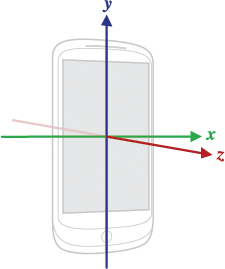
\includegraphics[width=0.20\linewidth]{./img/axis_magnetic_field.png}
	\caption{Assi x, y, z centrati sul cellulare}
	\label{fig:axis_magnetic_field}
\end{figure}


I tre valori sono espressi in $ \mu T $ (micro Tesla), unita' di misura della densita' di un flusso magnetico.
Le onde magnetiche raccolte sono dati continui sia positivi che negativi. L'intensita' dell'onda deriva dalla distorsione del campo magnetico generata dagli oggetti statici intorno al punto e dipende anche dalla velocita' con cui ci muoviamo per cui, per semplicita', assumeremo d'ora in poi una velocita' costante di 3 piedi al secondo.

\begin{figure}[H]
	\centering
	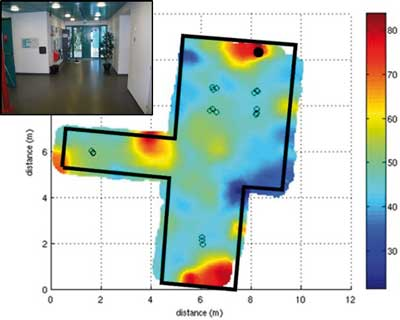
\includegraphics[width=0.7\linewidth]{img/magnetic_field_map}
	\caption[Un esempio di mappa del campo magnetico]{Mappa del campo magnetico all'universita' di Oulu: Discus Entrance hall}
	\label{fig:magneticfieldmap}
\end{figure}

\subsection{Estrazione del magnitudo}
Per estrarre l'intensit\`{a} di ogni onda magnetica eseguiamo semplicemente la norma euclidea di un vettore:\\
\begin{center}
	$ \sqrt{x^2 + y^2 + z^2}$
\end{center}

\subsection{Raggruppamento}
Le onde magnetiche con la stessa \textit{label} vengono raggruppate in \textit{fingerprints}, insiemi di dimensione prefissata. A livello logico, ogni \textit{fingerprint} cerca di identificare univocamente un punto all'interno di una zona, identificata con una \textit{label}. L'insieme di \textit{fingerprints} quindi, cerca di distinguere, tramite le caratteristiche dei campi elettromagnetici di ciascun punto, ogni \textit{label} dall'altra.

\subsection{Estrazione degli attributi}
Per ogni \textit{fingerprint}, l'estrazione delle \textit{features} consiste nell'estrazione di variabili statistiche. In questo specifico caso sono:
\begin{itemize}
	\item Media
	\item Varianza
	\item Deviazione standard
	\item Mediana
	\item Media troncata
	\item Coefficiente di variazione
	\item Massimo
	\item Minimo
	\item $ 1^{\circ}, 5^{\circ}, 95^{\circ}, 99^{\circ} $ percentile
	\item $ 1^{\circ}, 2^{\circ}, 3^{\circ} $ quartile
\end{itemize}





\section{Fase 2: costruzione di un modello}

Dopo aver raccolto ed elaborato le onde magnetiche, un algoritmo creera' un classificatore in grado di assegnare un'etichetta ai nuovi input ricevuti durante l'uso dell'utente finale.
Sono stati utilizzati vari classificatori per cercare il piu' preciso fra tutti. Qui di seguito introdurremo la teoria dietro ad ogni classificatore utilizzato.
\newpage
\subsection{IA ed Apprendimento}
La definizione secondo wikipedia \footnote{\url{https://it.wikipedia.org/wiki/Intelligenza_artificiale}} di IA e' la seguente:\\

Definizioni specifiche possono essere date focalizzandosi o sui processi interni di ragionamento o sul comportamento esterno del sistema intelligente ed utilizzando come misura di efficacia o la somiglianza con il comportamento umano o con un comportamento ideale, detto razionale:
\begin{itemize}
	\item Agire umanamente: il risultato dell'operazione compiuta dal sistema intelligente non e' distinguibile da quella svolta da un umano.
	\item Pensare umanamente: il processo che porta il sistema intelligente a risolvere un problema ricalca quello umano. Questo approccio � associato alle scienze cognitive.
	\item Pensare razionalmente: il processo che porta il sistema intelligente a risolvere un problema � un procedimento formale che si rif� alla logica.
	\item Agire razionalmente: il processo che porta il sistema
\end{itemize} 
L'apprendimento automatico e' una branca dell'intelligenza artificiale che permette al computer di apprendere da insiemi di dati per generare conoscenza con lo scopo di effettuare previsioni.

\subsection{Tipi di apprendimento}
Esistono 3 tipi di apprendimento:
\begin{itemize}
	\item Apprendimento supervisionato: al calcolatore vengono forniti esempi del tipo (\textbf{x}, y) per poter apprendere. L'obbiettivo della predizione per nuovi input sara' quello di calcolare la variabile dipendente. Y puo' essere sia dicreta che continua: nel primo caso si parla di classificazione, nel secondo di regressione.
	
	
	\begin{figure}[H]
		\centering
		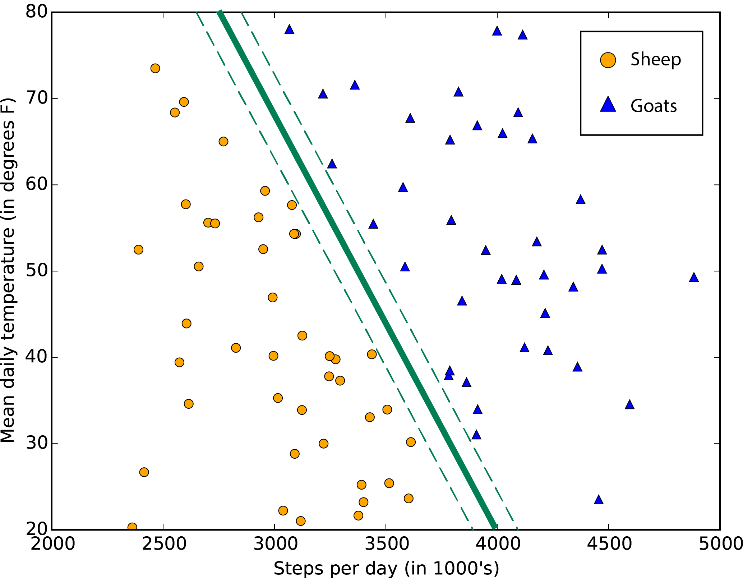
\includegraphics[width=0.7\linewidth]{img/supervised_learning_example}
		\caption{Un esempio grafico di insieme d'addestramento ed una sua classificazione}
		\label{fig:supervisedlearningexample}
	\end{figure}
	
	
	\begin{figure}[H]
		\centering
		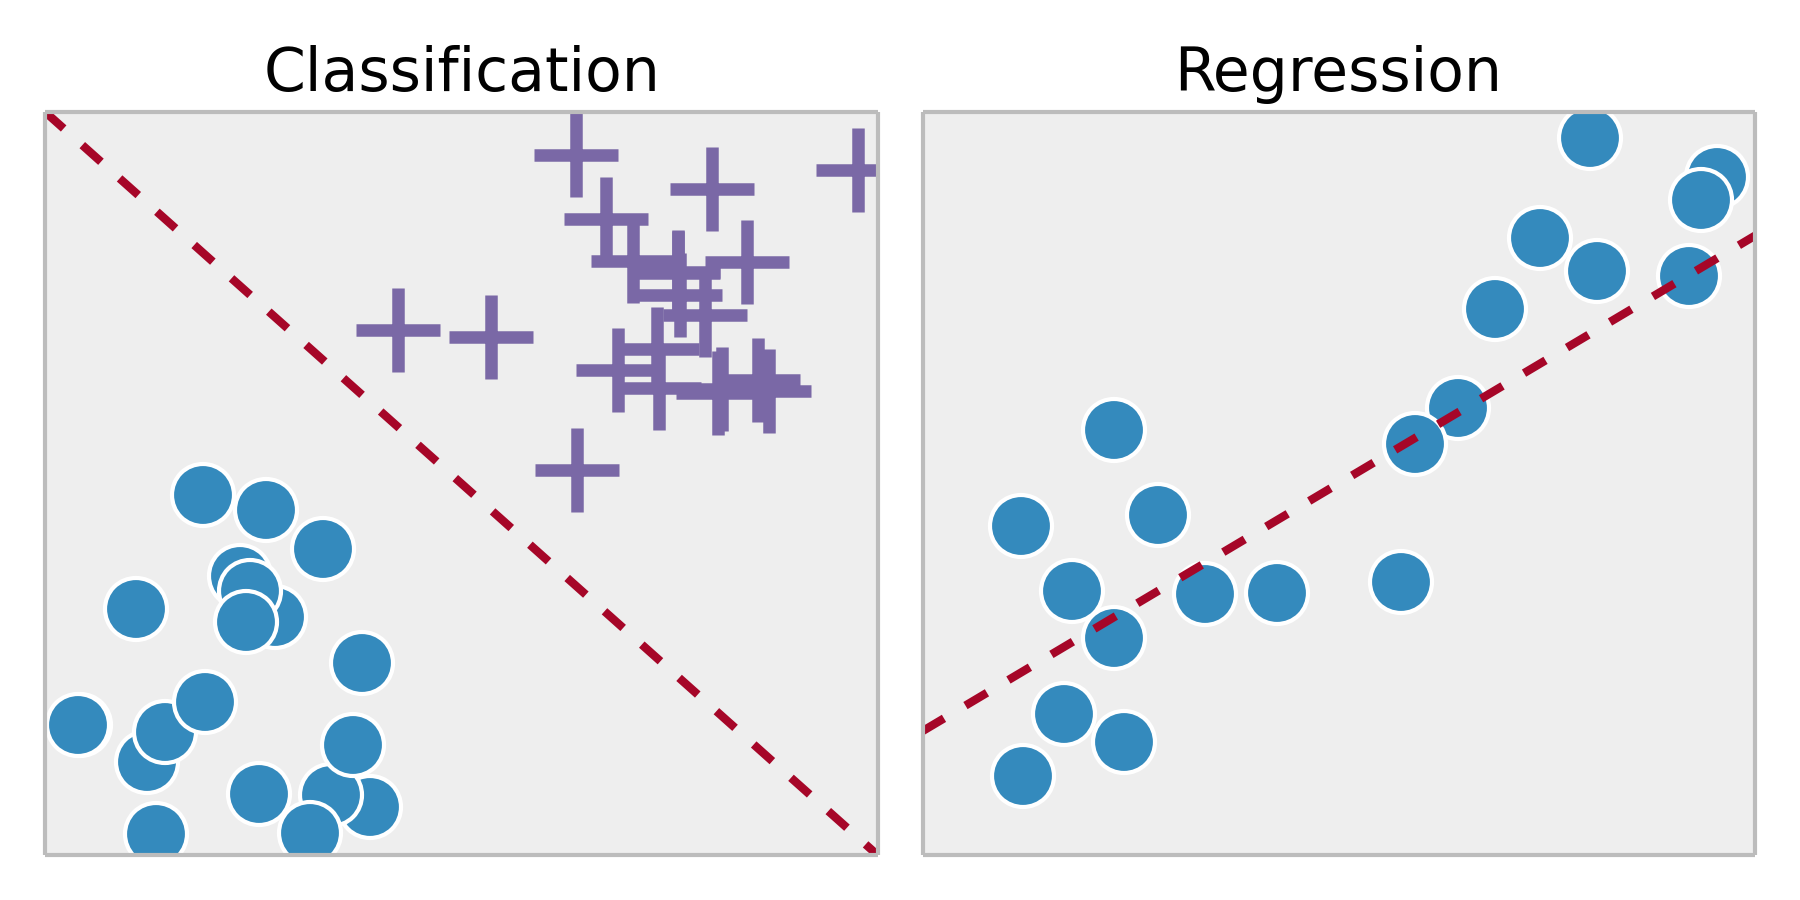
\includegraphics[width=0.7\linewidth]{img/Classification_Regression}
		\caption{Classificazione e regressione a confronto}
		\label{fig:classificationregression}
	\end{figure}

	\item Apprendimento non supervisionato: Gli esempi non contengono una variabile dipendente ma solo un insieme di attributi \textbf{x}. L'obbietto e' quello di inferire pattern nascosti dai dati non etichettati. Un'importante applicazione e' il \textit{clustering}: raggruppare i dati in base ad una similarita' fra di essi.
	
	\begin{figure}[H]
		\centering
		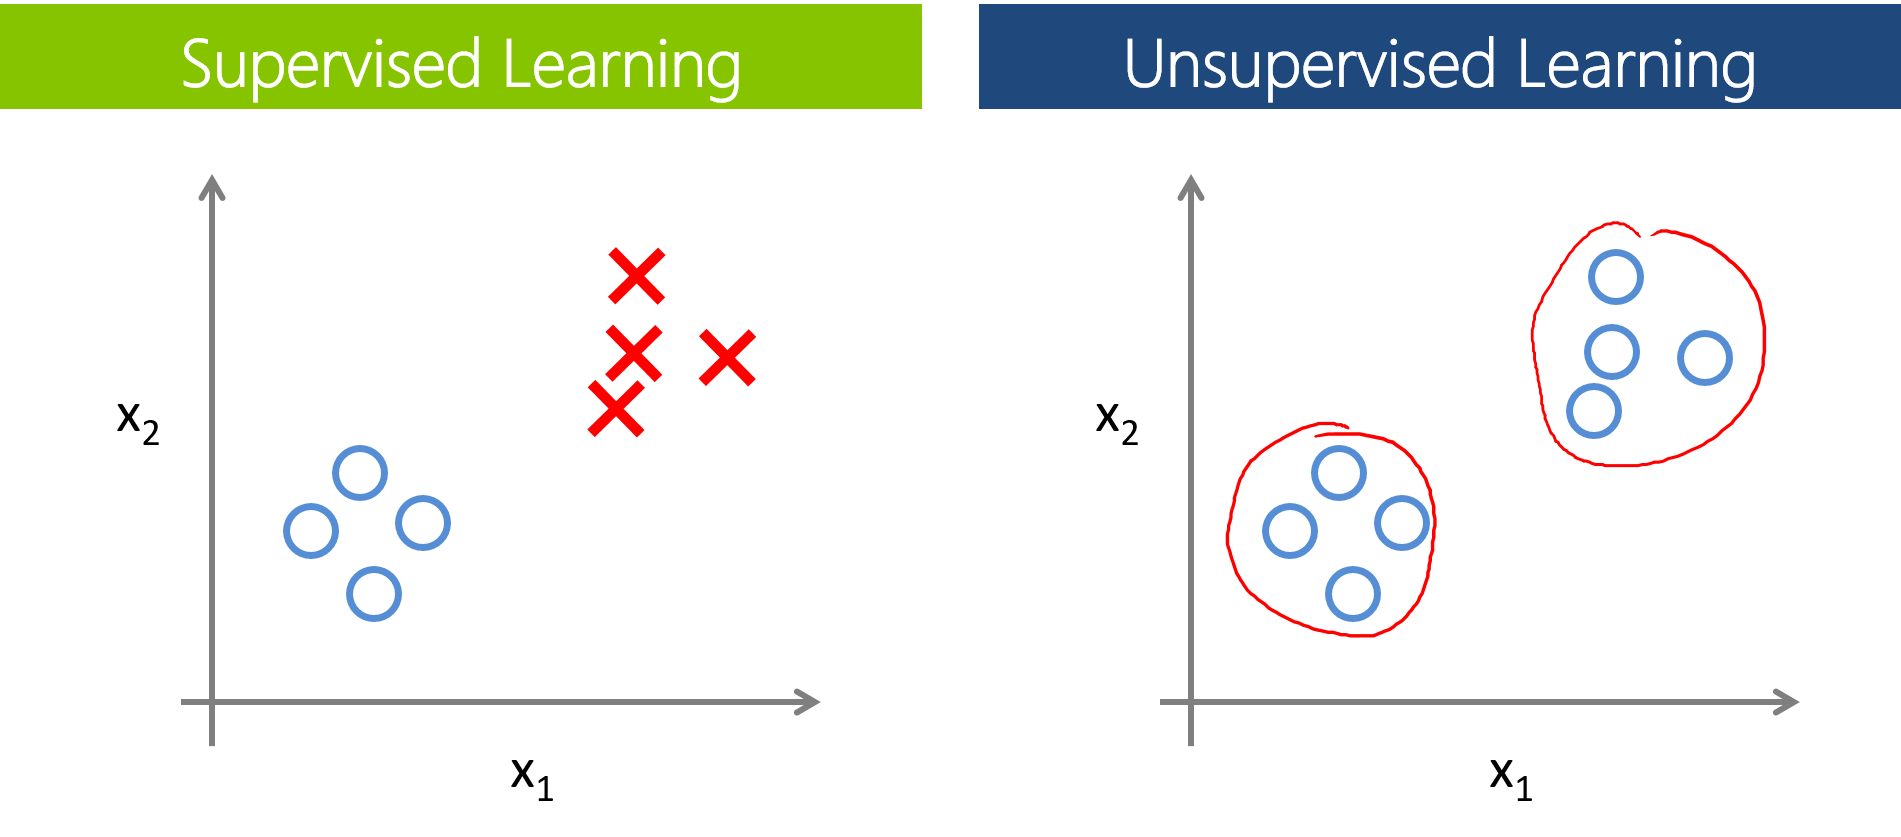
\includegraphics[width=0.7\linewidth]{img/supervised_and_unsupervised_learning}
		\caption{Apprendimento supervisiono e non supervisionato a confronto}
		\label{fig:supervisedandunsupervisedlearning}
	\end{figure}
	
	
	\item Apprendimento con rinforzo: per apprendere viene fornita una funzione ricompensa cioe' una funzione che, data un'azione effettuata dall'agente, restituira' una ricompensa di tipo numerico.
	
	\begin{figure}[H]
		\centering
		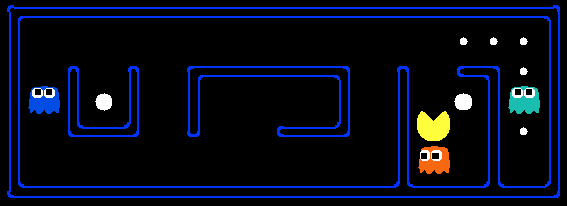
\includegraphics[width=0.7\linewidth]{img/pacman}
		\caption{L'apprendimento con rinforzo e' molto adatto ai giochi, come per esempio pacman}
		\label{fig:pacman}
	\end{figure}
	
	
\end{itemize}


\subsection{Alcune nozioni sull'apprendimento automatico}
\subsubsection{Verifica delle prestazioni}
Per verificare la correttezza del classificatore viene diviso in 2 parti il \textit{dataset} a nostra disposizione: il primo si chiama insieme di addestramento mentre il secondo insieme di test. Il nostro classificatore si allenera' sull'insieme di addestramento, cioe' imparera' dagli esempi come classificare i nuovi input e verifichera' l'efficacia dell'apprendimento sugli esempi in base ad una metrica. Ne esistono diverse ma noi useremo l'accuratezza, ovvero il numero di classificazioni corrette diviso il numero di esempi nell'insieme di test

\begin{figure}[H]
	\centering
	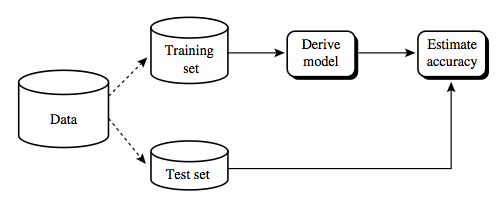
\includegraphics[width=0.7\linewidth]{img/training_test_flow}
	\caption{Un diagramma di flusso che mostra le operazioni di verifica delle prestazioni}
	\label{fig:trainingtestflow}
\end{figure}

\subsubsection{Parametri ed iperparametri}
Ogni modello e' composto da 2 tipi di valori che ne stabiliscono l'efficacia: i parametri, i quali sono determinati internamente dal modello in base al dataset mentre gli iperparametri sono stabiliti dall'utente prima dell'addestramento del modello e  modificano profondamente l'efficacia di predizione. Un esempio che vedremo e' l'iperparametro $k$ del $knn$.




\begin{figure}[H]
	\centering
	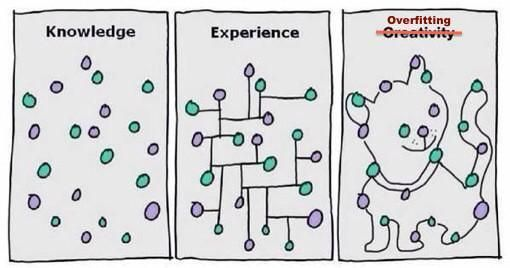
\includegraphics[width=0.7\linewidth]{img/overfitting}
	\caption{Effetti del sovradattamento}
	\label{fig:overfitting}
\end{figure}

\subsubsection{Insieme di validazione}
Per poter stimare il miglior valore da assegnare ai iperparametri del nostro modello, e' opportuno creare un altro insieme dal nostro dataset di partenza: l'insieme di validazione. Notiamo che non e' possibile utilizzare l'insieme di test per questo scopo perche' incapperemo in sovradattamento.

\subsubsection{Cross validation}
Un'alternativa all'insieme di validazione, specie se abbiamo un dataset piccolo, potrebbe essere la \textit{cross validation}. Inizialmente si suddivide l'intero dataset in $n$ parti (di solito 10). A turno una singola parte svolgera' il ruolo di insieme di validazione mentre tutto il resto sara' l'insieme di addestramento. Per valutare le prestazioni verra' fatta una media dell'accuratezza nelle predizioni in modo da avere un risultato piu' preciso rispetto al singolo insieme di validazione. Questa tecnica e' anche utile per evitare sovradattamento sui dati.

\begin{figure}[H]
	\centering
	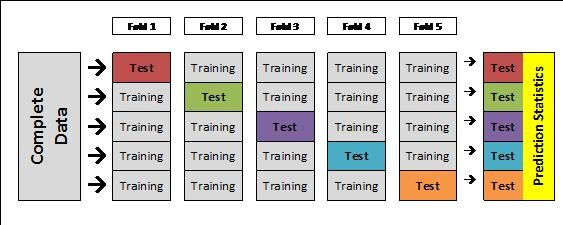
\includegraphics[width=0.7\linewidth]{img/crossvalidation}
	\caption{Rappresentazione grafica della Cross Validation}
	\label{fig:crossvalidation}
\end{figure}

\subsubsection{Rumore e sovradattamento}
Un problema molto comune durante l'addestramento dei classificatori e' il rumore: durante la discriminazione degli esempi, ci potrebbe capitare di avere vari esempi con attributi identici ma con etichetta differente. Una probabile causa potrebbe essere la presenza di errori nei dati mentre una possibile soluzione e' il voto di maggioranza fra gli esempi rimanenti.\\
Un'altro problema e' il sovradattamento: la costruzione di un classificatore consistente con tutti gli esempi porta ad inaccuratezza nei casi reali d'uso. Una possibile causa e' l'utilizzo di attributi irrilevanti nella classificazione. Supponiamo di voler predire l'esito del lancio di un dado e fra gli attributi di avere ora, giorno, mese ed anno; ecco un esempio lampante di sovradattemento. Nei casi reali tuttavia non sono cosi' evidenti gli attributi insignificanti e, per esempio, una tecnica utilizzata  negli alberi di decisione e' la potatura.

\subsection{K Nearest Neightbour}
Uno degli algoritmi piu' semplici di apprendimento automatico, e' il \textit{k-nearest-neightbours} dove l'input consiste in $k$ elementi presi dal \textit{training set} piu' vicini in base ad un criterio scelto da chi utilizza l'algoritmo (per esempio la distanza euclidea o di Mahalanobis). Il KNN viene definito un algoritmo pigro (\textit{lazy}) perche' non ha bisogno di apprendere dall'insieme di addestramento per poter creare un classificatore ma puo' usare direttamente i dati forniti per classificare i nuovi esempi. Questo vantaggio ha un prezzo da pagare: durante la predizione abbiamo una complessita' di tempo proporzionale alla grandezza del dataset.


\begin{figure}[H]
	\centering
	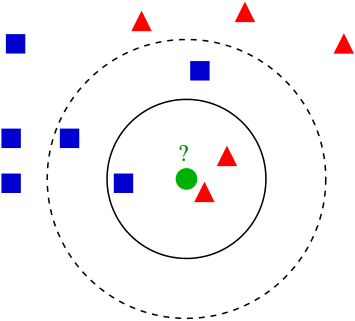
\includegraphics[width=0.7\linewidth]{img/knn_example}
	\caption{Esempio grafico dell'algoritmo KNN}
	\label{fig:knnexample}
\end{figure}


\subsubsection{Scelta del parametro k}
La scelta del parametro dipende, ovviamente, dal tipo dei dati che abbiamo e dalla quantita', anche se in generale piu' e' grande $k$ meno rumore viene generato da questo algoritmo. Un buon metodo per trovare il giusto valore e' l'uso di tecniche euristiche, come la \textit{cross validation}. Un altra fonte di rumore di cui bisogna stare attenti e' la presenza di \textit{features} insignificanti nella ricerca del vicino. Per porre rimedio possiamo, ad esempio, usare un algoritmo genetico per selezionare le \textit{features} piu' significative

\subsubsection{\textit{Curse of dimensionality}}
Un problema di cui soffrono vari modelli fra cui $knn$ e' la maledizione della dimensionalita' ovvero quando abbiamo dataset con elevata dimensionalita' come 50 attributi, modelli come $knn$ diventano molto imprecisi. Nel nostro classificatore la motivazione e' semplice: con tanti attributi la distanza tra punti incorrelati fra loro potrebbe diventare bassa soprattuto se presente del rumore nei dati oppure attributi insignificanti. Nel nostro problema non soffriamo della maledizione della dimensionalita' perche' abbiamo solo 3 attributi.

\subsection{Naive bayes}
Un altro tipo di apprendimento usato per classificare le \textit{label} e' Naive bayes: un algoritmo di classificazione e regressione basato sulla statistica. Prima di spiegare in cosa consiste occorre spiegare un paio di concetti:
\subsubsection{Teorema di bayes}
Il teorema di bayes ci fornisce una relazione fra probabilita' condizionate molto utile nel calcolo probabilistico ma anche per l'apprendimento automatico. L'equazione e' la seguente:
\begin{center}
	$P(B|A) = \dfrac{P(A|B)P(B)}{P(A)}$
\end{center}
\subsubsection{Rete bayesiana}
Una rete bayesiana e' un grafo diretto aciclico i cui nodi sono le variabili casuali del sistema mentre gli archi rappresentato la condizione di dipendenza fra nodi.
 Ad ogni nodo e' associata una tabella di distribuzione delle probabilita' la cui complessita' e' proporzionale al numero di archi entranti.\\ Per esempio se il nodo con variabile casuale Leggere ha un arco verso Istruito allora possiamo dire che Istruito e' condizionalmente dipendente da Leggere. Qui sotto potete vedere una raffigurazione grafica di una semplice rete bayesiana formata da nodi padre ed un figlio:
\begin{figure}[H]
	\centering
	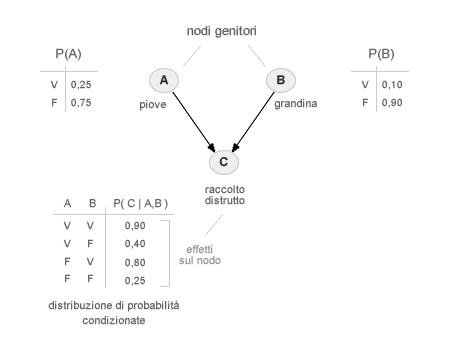
\includegraphics[width=0.7\linewidth]{img/rete-bayesiana-grafo.png}
	\caption{Esempio di rete bayesiana}
	\label{fig:rete-bayesiana-grafo}
\end{figure}
\medskip
\subsubsection{Naive Bayes}
Naive bayes e' una rete bayesiana in cui si assume l'indipendenza condizionale fra tutte le variabili casuali del sistema data la classe. Questa forte assunzione non mira a modellare esattamente la realta' ma nonostante cio' fornisce delle buone performance sulla predizione di una classe.

\begin{figure}[H]
	\centering
	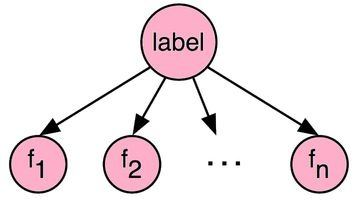
\includegraphics[width=0.4\linewidth]{img/naive_bayes_example}
	\caption{Esempio di rete bayesiana ingenua}
	\label{fig:naivebayesexample}
\end{figure}

\medskip
\subsubsection{Predizione di risultati}
Preso un insieme di attributi $\textbf{x}$ con valori $x_1x_2x_3...x_n$ e tutti i valori possibili della variabile dipendente $\textbf{y}=y_1y_2y_3...y_m$ , per classificare l'insieme applicheremo il teorema di bayes con un'approssimazione molto usata nel campo scientifico chiamata MAP (Massima ipotesi a posteriori)
\begin{align*}
		etichetta &=y_j \, in \, \max_j\,P(y_j|X_1=x_1, X_2=x_2...X_N=x_n) \\
		&= \max_j \dfrac{P(X_1=x_1,X_2=x_2...X_N=x_n|y_j)P(y_j)}{P(X_1=x_1, X_2=x_2...X_N=x_n)}\\
		&= \max_j \dfrac{\prod_iP(x_i|y_j)P(y_j)}{P(X_1=x_1, X_2=x_2...X_N=x_n)}
\end{align*}

i cui valori della precedente equazione si possono ricavare dalla tabella di distribuzione delle probabilita'.

\subsubsection{Modelli generativi e discriminativi}
Una distinzione fra classificatori e' possibile farla nel modo in cui viene calcolata l'espressione $P(y_j|\textbf{x})$: nel caso di modelli discriminativi  (ad esempio \textit{knn} e alberi di decisione), l'obbiettivo e' discriminare, cioe' suddividere i dati originale per poter assegnare un'etichetta ai nuovi input mentre nei modelli generativi) l'obbiettivo e' di generare una distribuzione congiunta di probabilita' per $P(\textbf{x}, y_j)$ oppure da $P(\textbf{x}| y_j)$ e $P(y_j)$ per poter trovare l'etichetta piu' probabile. Fra questi ultimi ricade \textit{Naive Bayes}.

\subsubsection{Calcolo della probabilita' a priori}
  Per calcolare la probabilita' a priori esistono varie tecniche: l'equiprobabilita' $\left(\dfrac{1}{|\textbf{y}|}\right)$, rapporto fra esempi di classe $j$ e il totale degli esempi dall'insieme di addestramento, modelli ad eventi oppure un modello non parametrico dall'insieme di addestramento.
  
\subsubsection{Modelli ad eventi}  
   I modelli ad eventi sono distribuzioni di probabilita' che considerano gli attributi come probabilita' di eventi. Ci sono 3 modelli usati con $\textit{Naive Bayes}$ che sono:
\begin{itemize}
	\item Bernoulli: gli attributi sono di tipo \textit{booleano} e l'attributo $x_i \in \textbf{x}=(x_1,x_2,...,x_n)$ vale 1 se l'evento $i$ e' avvenuto, 0 altrimenti. Nel caso bernoulliano possiamo valutare $P(\textbf{x}|y_j)$ come
	\begin{center}
	 $P(\textbf{x}|y_j) = \prod_{j=1}^{n} P_{ij}^{x_i} (1-P_{ij})^{(1-x_i)}$
	\end{center}
	Dove $P_{ij}$ e' la probabilita' per $y_j$ che $x_i$ sia vero. Un esempio canonico e' quello della classificazione dei documenti, dove $x_i$ rappresenta la presenza del termine $w_j$ nei documenti di classe $y_j$ e di conseguenza $P_{ij}$ la probabilita' di trovarlo. Dobbiamo notar bene che Bernoulli a differenza della multinomiale valuta nella produttoria anche la probabilita' che l'evento $i$ non avvenga.
	

	\item Multinomiale: Nella multinomiale gli esempi rappresentano la frequenza con il quale gli eventi sono stati generati dalla multinomiale $(p_1...p_n)$ dove $p_i$ e' la probabilita' che $i$ occorra. Gli attributi $\textbf{x}=(x_1,x_2...x_n)$ contano quante volte l'evento $i$ e' avvenuto. La probabilita' condizionata  $P(\textbf{x}|y_j)$ e' stimata come
	\begin{center}
		$P(\textbf{x}|y_i) = \dfrac{(\sum_{i}x_i)!}{\prod_{i}x_i!}\prod_i p_{ki}^{x_i}$
	\end{center}
	\item Gaussiana: viene utilizzata con dati continui e si assume che siano distribuiti in base alla Gaussiana. Per ogni classe $y_j$, viene ricavata la media $\mu_j$ e la varianza $\sigma_{j}^{2}$. Supponiamo di aver raccolto un insieme di valori $v$ allora la probabilita' sara':
	\begin{center}
		$P(x =v | y_j) = \dfrac{1}{\sqrt{2 \pi \sigma_{j}^2}} e^{-\dfrac{(v - \mu_j)^2}{2 \sigma_{j}^2}}$
	\end{center}
	Un'altra possibile opzione per trattare valori continui e' la discretizzazione da cui possiamo utilizzare Bernoulli/Multinomiale anche se bisogna stare attenti a non perdere informazioni discriminanti.
\end{itemize}

\subsubsection{Un piccolo esempio basato su naive bayes}
Supponiamo di dover usare Naive Bayes per predire se giocare una partita di tennis o no in base alle condizioni meteorologiche. Dati gli esempi qui sotto a sinistra, possiamo ricavare la tabella di distribuzione delle probabilita' generale come qui di seguito:
\begin{figure}[H]
	\centering
	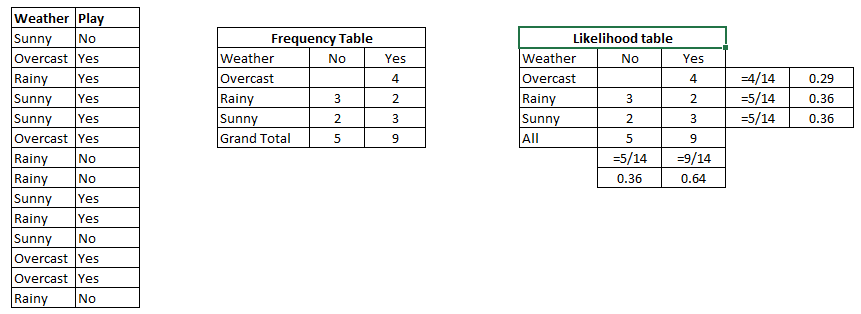
\includegraphics[width=1\linewidth]{img/Bayes_tennis_sample}
	\caption{Esempi di partite di tennis giocate in base alle condizioni meteorologiche e tabella di distribuzione delle probabilita'}
	\label{}
\end{figure}
\medskip
Ecco una rappresentazione grafica di \textit{Naive Bayes}:\\\\

\begin{figure}[H]
	\centering
	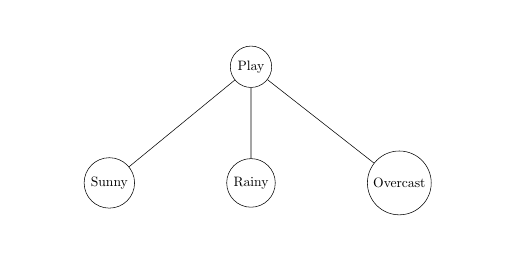
\includegraphics[width=0.7\linewidth]{img/graph_naive_bayes}
	\caption{Rappresentazione grafica di \textit{Naive bayes} nell'esempio del tennis}
	\label{fig:graphnaivebayes}
\end{figure}

%	\begin{tikzpicture} 
%		\node[draw, circle](0){Play}
%		child{ node(1)[draw, circle, left]{Sunny}}
%		child{	 	node(2)[draw, circle]{Rainy}}
%		child{	  node(3)[draw, circle, right]{Overcast} };
%	\end{tikzpicture}
\subsection{Alberi di decisione}
Da un punto di vista strutturale, l'albero di decisione e' un albero (inteso come struttura dati) dove i nodi interni sono gli attributi, i rami tutti i possibili valori assumibili dall'attributo (oppure un range nel caso continuo) e le foglie sono la predizione da scegliere.

\subsubsection{Classificazione dei nuovi elementi}
Quando dovremmo predire l'etichetta di un nuovo insieme di attributi $x$ bastera' semplicemente scorrere l'albero di decisione dalla radice fino ad una foglia, che sara' l'etichetta da assegnare.

\begin{figure}[H]
	\centering
	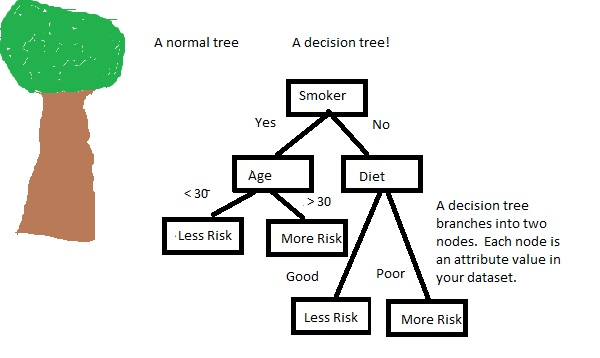
\includegraphics[width=0.7\linewidth]{img/dectree}
	\caption{Un albero e un albero di decisione a confronto. Nel secondo abbiamo come attributi \textit{Smoker, Age, Diet} e come etichetta \textit{Less Risk, More Risk} riferito alle malattie cardiache. }
	\label{fig:dectree}
\end{figure}


\subsubsection{Costruzione di un albero di decisione}
La costruzione dell'albero e' molto semplice: basta prendere gli attributi ed iniziare a suddividere a caso fino ad ottenere nodi con esempi di un solo tipo di etichetta.
In questo modo pero' otterremmo un albero  non molto utile in tutti i casi diversi dagli esempi. Quindi quale albero scegliere fra tutti quelli possibili? In questo caso ci aiuta un principio filosofico, il rasoio di Occam, che ci consiglia di scegliere quello piu' piccolo fra tutti. Per generare l'albero piu' piccolo dovremmo scegliere gli attributi piu' significativi per generare l'albero. Cosa intendiamo per significativo? Intendiamo l'attributo che genera figli con meno varieta' di classi presenti all'interno di essi, cioe' che discrimina meglio degli altri.\\ Un esempio: immaginiamo di avere 10 esempi con attributi A e B e come etichetta ${0,1}$. Ipotizziamo che suddividendo tramite l'attributo A avremmo due figli con esempi aventi meta' valore 0 e meta' 1 mentre se suddividiamo secondo B abbiamo nodi figli con esempi esclusivamente 1 oppure 0. In questo caso indubbiamente l'attributo piu' significativo e' B.\\Esistono vari criteri per misurare l'attributo piu' significato su cui suddividere il nodo che in termini tecnici vengono chiamate misure d'impurita'. Una misura e' l'indice di Gini il quale corrisponde alla seguente formula:
\begin{center}
	$\sum_{j} p(j|n)(1-p(j|n))$
\end{center}
dove $p(j|n)$ e' la percentuale di esempi con classe $j$ nel nodo $n$


\subsubsection{Un esempio di albero di decisione}
Riprendiamo l'esempio della partita di tennis, questa volta con qualche attributo in piu'. La tabella e' la seguente:
\begin{figure}[H]
	\centering
	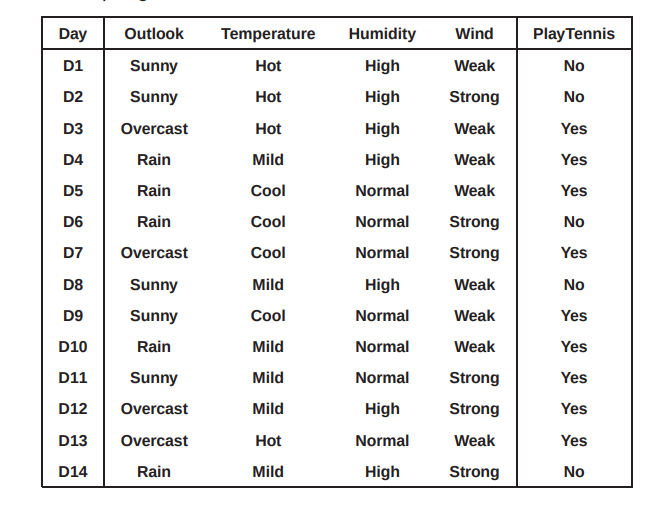
\includegraphics[width=0.7\linewidth]{img/decision-_tree_table_tennis}
	\caption{Tabella degli attributi meteorologici con valore associato un booleano che stabilisce se la partita e' stata giocata o no}
	\label{fig:decision-treetabletennis}
\end{figure}
da cui possiamo ricavare il seguente albero di decisione:
\begin{figure}[H]
	\centering
	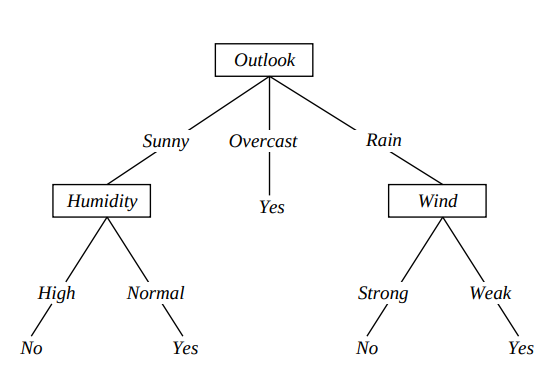
\includegraphics[width=0.7\linewidth]{img/decision_tree_tree_tennis}
	\caption{Albero di decisione ricavato dalla tabella precedente}
	\label{fig:decisiontreetreetennis}
\end{figure}

\section{Fase 3: Ricerca della posizione}
Dopo la costruzione del modello esso viene adoperato per predire la posizione corrente dell'utente che esegue l'applicazione. La ricerca consiste nel creare sul momento una \textit{fingerprint} e poi, tramite un algoritmo di classificazione, cercare di inferire la \textit{label}  su cui ci troviamo. Gli algoritmi utilizzati per analizzare il problema sono quelli descritti in precedenza quindi
\begin{enumerate}
	\item \textit{K Nearest Neightbour}
	\item Bayes ingenuo
	\item  Alberi di decisione
\end{enumerate}
\newpage

\chapter{Struttura del software}

\section{Linguaggi e librerie}
L'applicazione ha come \textit{target platform} \textit{Android} perci\`o il linguaggio usato principalmente \`e stato \textit{Java}. Da notare che su \textit{Android} il linguaggio \`e presente nella versione 7, perci\`o non sono disponibili alcune funzionalit\`a di \textit{Java} 8 come i metodi di default, \textit{stream}, \textit{lambda expression} ecc. Sono state usate delle librerie esterne fra i quali \textit{Gson} che consente la serializzazione/de-serializzazione dei dati, \textit{lombok} che fornisce delle annotazioni che abbreviano il codice mantenendo una buona espressivit\`a, varie librerie di supporto \textit{Android} ed una libreria \textit{Apache} che fornisce molte utilit\`a matematiche. Mosso dalla curiosit\`a, ho provato ed alla fine utilizzato nel progetto \textit{Kotlin}, un linguaggio che compila in \textit{bytecode} per la JVM $100 \%$ interoperabile con \textit{Java} 6 (e successivi) che, fra le varie cose, fornisce le funzionalit\`a sopracitate mancanti a \textit{Java} 7.

\section{Applicazione}
L'applicazione ha lo scopo di catturare le onde magnetiche all'interno di un edificio tramite il magnetometro, un sensore presente ormai su tutti gli \textit{smartphone}. A livello di codice, per poter ricevere le onde magnetiche dal magnetometro \`e necessario una istanza di una sottoclasse dell'interfaccia \textit{SensorListener} od una classe anonima, che vuol dire creare un'implementazione dei metodi astratti sul momento. Il termine anonima deriva dal fatto che, a differenza delle sottoclassi, non viene assegnato un tipo nominale esplicitamente da parte del programmatore. L'istanza sottotipo di \textit{SensorListener} viene poi data input ad una funzione della libreria \textit{Android} che invier\`a  tramite notifiche \textit{push} le onde magnetiche rilevate dal magnetometro alla nostra classe. La scelta tra le due opzioni \`e ricaduta sull'implementazione di una sottoclasse di \textit{SensorListener} perch\'e la logica che ci sta dietro \`e abbastanza avanzata per una classe anonima. Il codice che implementa l'interfaccia  \`e il seguente:
\lstinputlisting[language=Java]{code/sensorlistener.java}
Sono state omesse alcune parti per non allungare ulteriormente il codice e concentrarci sulla parte essenziale della classe. Il metodo \textit{onSensorChanged} viene chiamato da \textit{Android} quando rileva un cambiamento nel campo magnetico. La condizione dentro l'\textit{if} ci permette di registrare le onde magnetiche ad intervalli regolari a patto che \textit{recordingRate} sia diverso da $-1$ (che rappresenta la  disattivazione della registrazione di onde ad intervalli regolari).
\\\\
Questo codice viene utilizzato sia durante la scansione dell'ambiente, cio\`e quando viene costruita per la prima volta la mappa delle distorsioni magnetiche all'interno dell'edificio, sia quando effettuiamo la ricerca della posizione dentro l'edificio.
\\\\
Ad ogni onda magnetica registrata viene assegnata un'etichetta, ovvero un numero intero rappresentante una zona della mappa che stiamo scansionando. Visto che in un secondo vengono raccolte molte onde magnetiche, quando ne abbiamo un numero abbastanza grande si creano delle \textit{fingerprint} che identificano un singolo punto della zona. Di solito un'etichetta identifica un'area (in genere una stanza) rispetto alla \textit{fingerprint} che rappresenta un singolo punto.
\\\\
Appena i dati sono stati raccolti, inizia la fase di preprocessamento dei dati. In questo caso non \`e stata fatta una normalizzazione/standardizzazione dei valori degli attributi perch\'e, tramite test empirici si \`e verificato che, portava ad una accuratezza pi\`u  bassa del $20\%$ circa. Da ogni \textit{fingerprint} sono state estratte nuove caratteristiche di natura statistica, tra le quali: Media, Varianza, Deviazione standard, Mediana, Media troncata, Coefficiente di variazione, Massimo, Minimo, $ 1^{\circ}, 5^{\circ}, 95^{\circ}, 99^{\circ} $ percentile, $ 1^{\circ}, 2^{\circ}, 3^{\circ} $ quartile.
Dopo non abbiamo una fase di addestramento del modello perch\'e nel codice su dispositivo \textit{Android} \`e stato usato il \textit{knn} e quindi c'\`e direttamente la fase di ricerca della posizione, od in termini pi\`u  tecnici per quanto riguarda l'apprendimento automatico, la predizione dell'etichetta.
\\\\
Adesso vediamo alcune statistiche sul codice \textit{Java}: il numero di righe \`e pari a 1443 linee di codice in 43 file quindi 43 classi od interfacce mentre con \textit{Kotlin} sono state scritte 742 linee di codice in 16 file.


\section{UML del codice}
Vediamo adesso un diagramma delle classi del codice \textit{Android} sviluppato. Sono state omesse alcune classi dall'UML perch\'e futili al fine di comprendere la struttura del programma.

\begin{figure}[H]
	\centering
	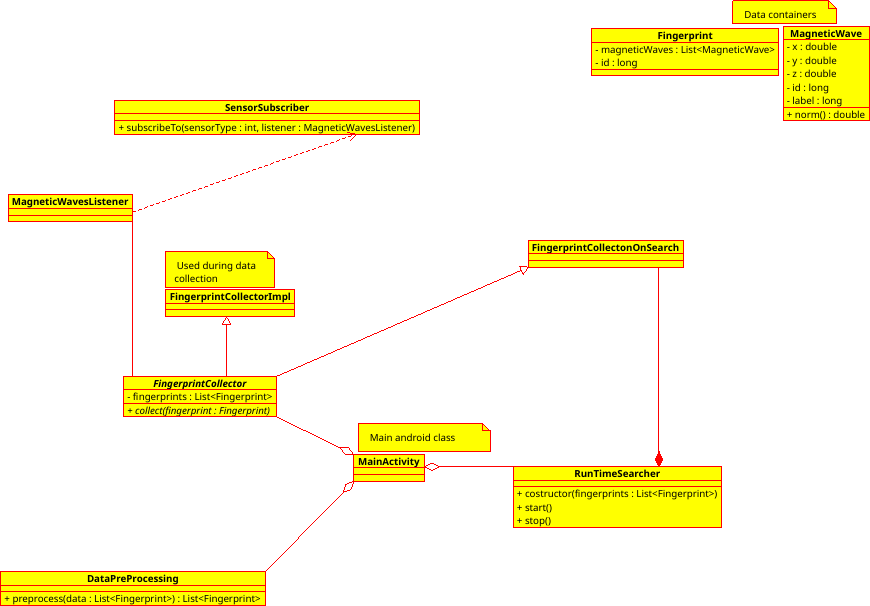
\includegraphics[width=1\linewidth]{img/class_diagram}
	\caption{Diagramma delle classi dell'applicazione}
	\label{fig:classdiagram}
\end{figure}

Al centro abbiamo la \textit{MainActivity}, che rappresenta per lo sviluppatore il "\textit{main}" del programma. In realt\`a non si tratta di una singola funzione di partenza, ma di tante che si attivano come reazione a certi eventi. Abbiamo fra le varie \textit{onCreate} che viene invocata all'avvio del programma, \textit{onPause, onResume} che si fanno intuire dal nome. \`E possibile trovare pi\`u informazione sulla vita dell'\textit{Activity} qua \footnote{\url{https://developer.android.com/reference/android/app/Activity.html}}.\\
Dalla \textit{MainActivity} partono 3 rami, ovvero 3 classi che compongono quest'ultima di cui uno per la raccolta di onde magnetiche, uno per il \textit{preprocessing} dei dati e l'ultimo per la ricerca della posizione dell'utente. In alto a destra invece abbiamo i 2 "contenitori dati" usati in tutto il programma.

\section{Interfaccia grafica}
L'interfaccia \`e stata realizzata ai fini di test pratici delle funzionalit\`a finali dell'applicazione quindi non ha una grande cura da un punto di vista estetico come vedremo pi\`u  avanti.
La parte alta mostra i 3 valori catturati tramite il magnetometro ed ottenuti dalle API di \textit{Android}. \\
Nel mezzo ci sono dei pulsanti per:
\begin{itemize}
	\item Iniziare/Terminare la scansione dell'ambiente.
	\item Incrementare la \textit{label} che viene assegnata alla prossima \textit{fingerprint} registrata. Il \textit{click} di questo bottone dovrebbe avvenire quando vogliamo cambiare zona da analizzare.
	\item Iniziare/Terminare la ricerca.
	\item Serializzare tutti i dati registrati dall'avvio dell'applicazione in formato \textit{JSON}
	\item De-serializzare i dati salvati.
\end{itemize}
Nella parte bassa invece c'\`e una \textit{textbox} contenente il \textit{log} che viene stampato durante l'esecuzione del programma.

\begin{figure}[H]
\centering
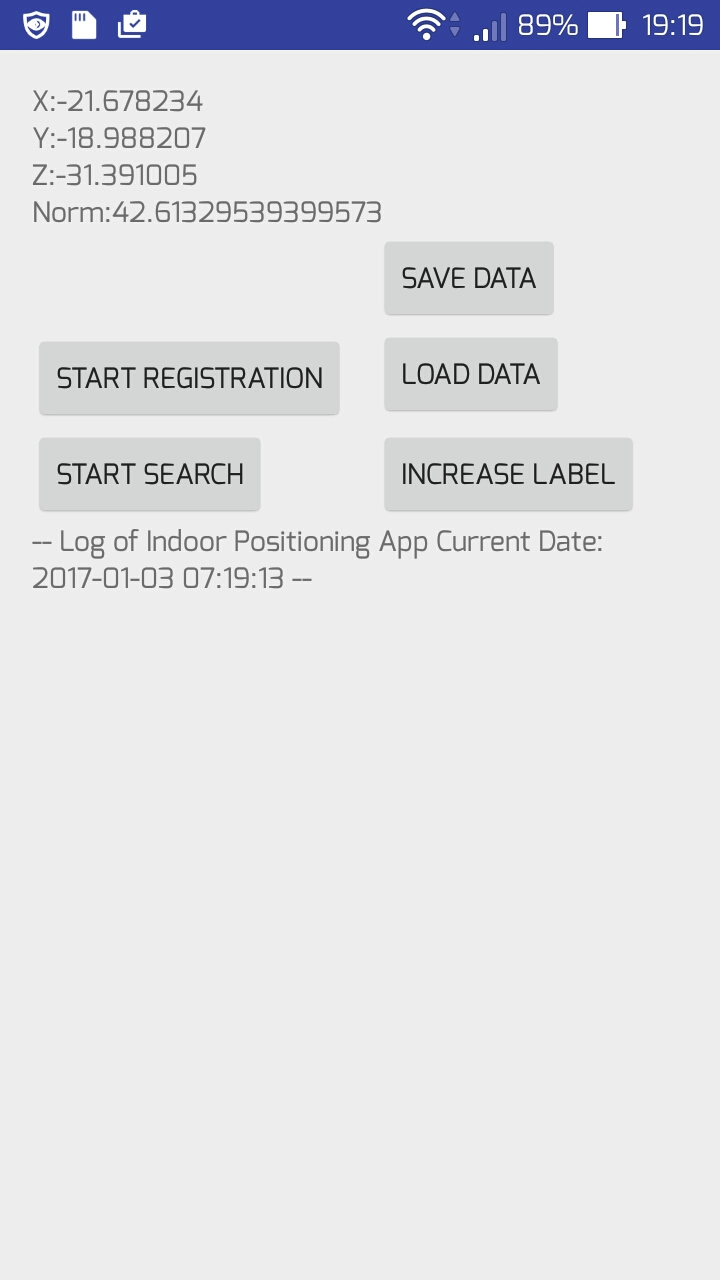
\includegraphics[width=0.4\linewidth]{img/app_screen}
\caption{Interfaccia grafica all'avvio dell'applicazione}
\label{fig:app_screen}
\end{figure}

\begin{figure}[H]
	\centering
	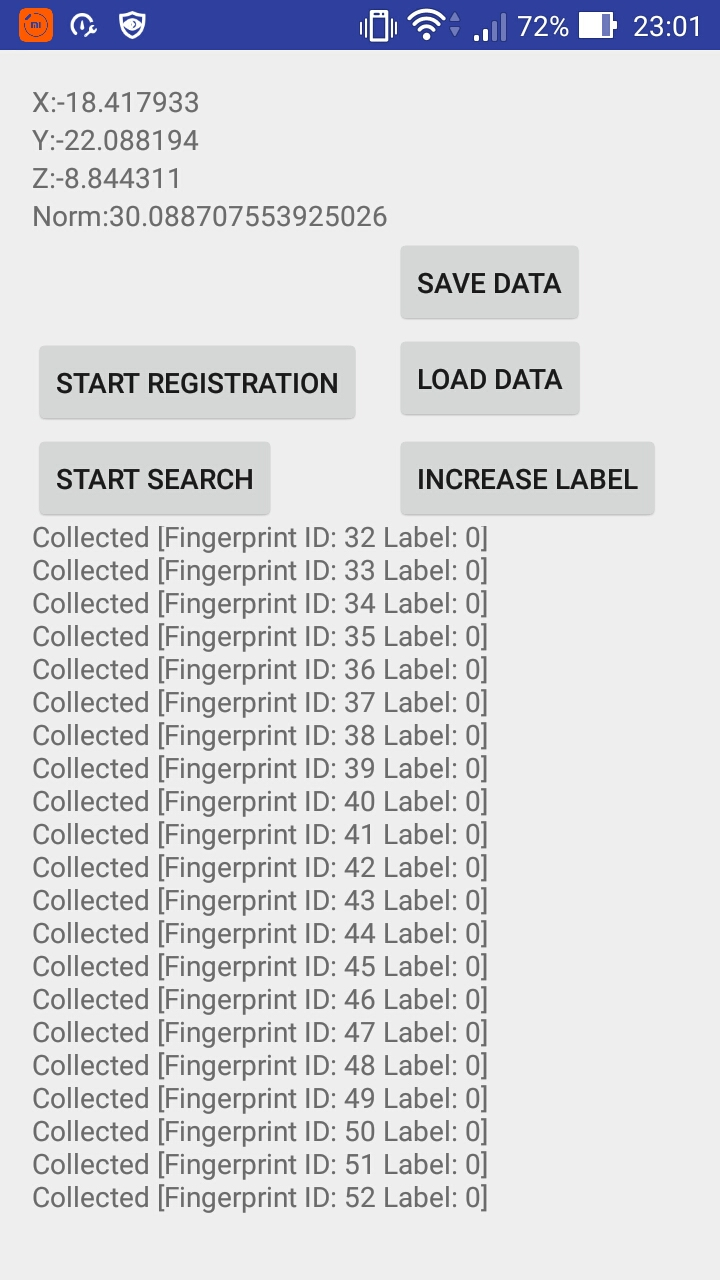
\includegraphics[width=0.4\linewidth]{img/app1}
	\caption{Immagine dell'applicazione durante la raccolta dati}
	\label{fig:app1}
\end{figure}

\begin{figure}[H]
	\centering
	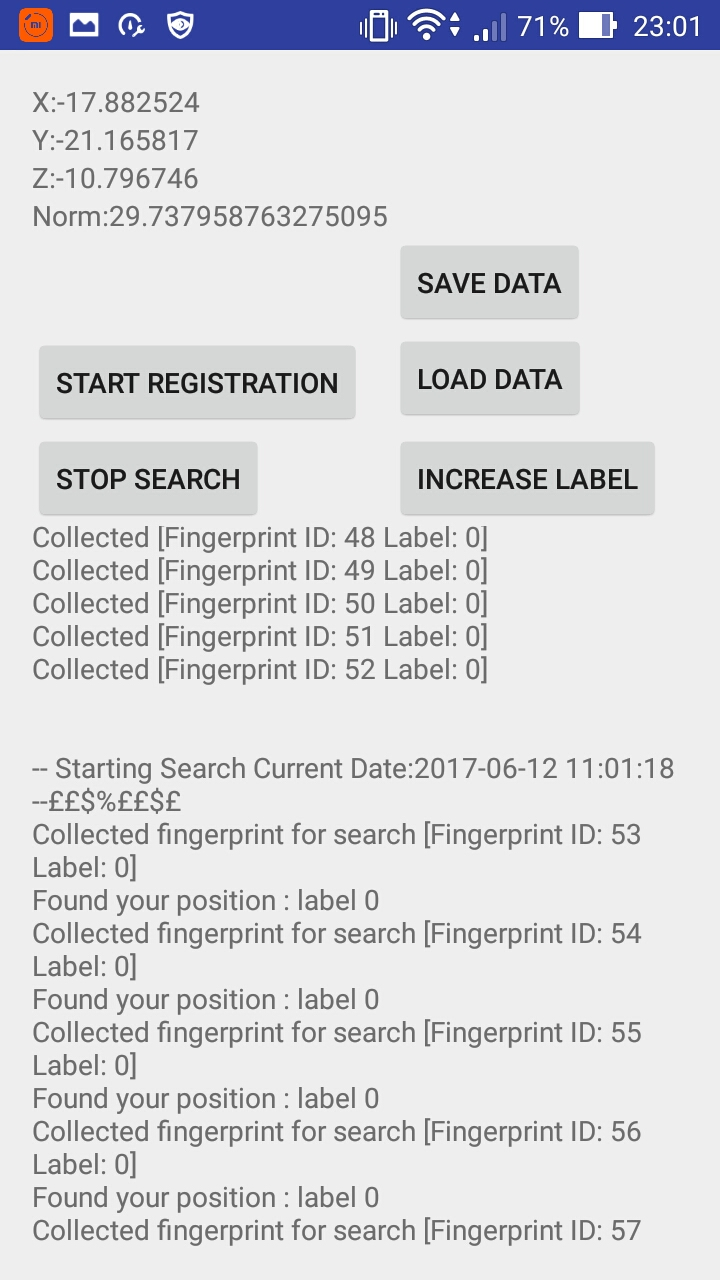
\includegraphics[width=0.4\linewidth]{img/app2}
	\caption{Immagine dell'applicazione durante la ricerca della posizione}
	\label{fig:app2}
\end{figure}


\section{Persistenza dei dati}
Innanzitutto spieghiamo che cos'\`e la serializzazione: \`e una procedura che consente di salvare su supporti di memorizzazione (\textit{hard disk}, chiavetta \textit{usb}) dei dati della nostra applicazione mentre la de-serializzazione \`e il procedimento inverso.
L'applicazione consente anche di serializzare tutti i dati registrati fino a quel momento nel formato standard \textit{JSON} tramite la libreria \textit{gson} che fornisce delle funzioni  per il linguaggio \textit{Java} per la serializzazione/de-serializzazione di oggetti. Il file viene salvato nella cartella dati dell'applicazione non visibile all'utente.

\section{Struttura del codice e design pattern}
Nello sviluppo del software sono stati applicati vari \textit{design pattern} e principi di programmazione visti durante i vari corsi. Fra questi ultimi abbiamo il \textit{dependency inversion principle}, \textit{open closed principle}. Riguardo i \textit{design pattern}, sono stati usati frequentemente l'\textit{observer}, il \textit{template} e \textit{factory}.


\chapter{Test}

\section{Analisi dei dati}
La predizione dei risultati \`e stata implementata sia nel software \textit{Android} sia sul computer. Nel codice eseguito su dispositivo mobile \`e stato adoperato solamente il KNN per via della facilita' d'implementazione e non \`e stato  utilizzato per testare la precisione, ma per verificare il corretto funzionamento dell'applicazione. Invece su computer, presi i dati serializzati dal software mobile, sono stati applicati tutti gli algoritmi di apprendimento elencati precedentemente e gia' tutti implementati da librerie di terze parti per verificare la precisione dei dati. Il linguaggio scelto su computer \`e \textit{Python} per via del suo buon supporto all' apprendimento automatico tramite la libreria \textit{sklearn}.



\section{Piano dei test}
Per testare l'effettivo funzionamento dell'applicazione ho usato alcune stanze di casa mia ed ho assegnato a ciascuna di esse una \textit{label}. Qui di seguito una piccola piantina rappresentante le stanze utilizzate:

\begin{figure}[H]
\centering
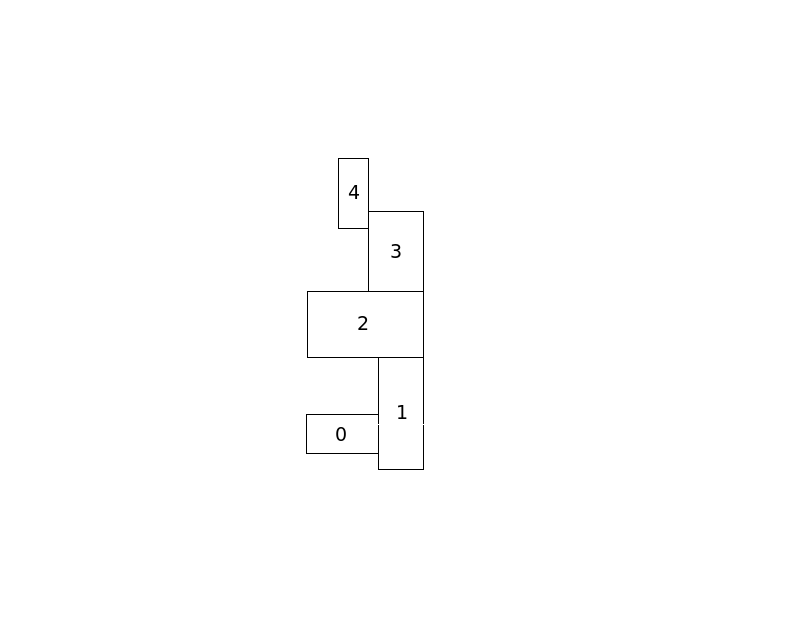
\includegraphics[width=0.7\linewidth]{img/test_pianta_casa}
\caption{Una piccola raffigurazione delle stanze usate per le prove con sopra scritto la \textit{label} assegnata}
\label{fig:test_pianta_casa}
\end{figure}

Sono stati raccolti circa 18000 campioni di onde magnetiche. La suddivisione fra addestramento e test \`e 70/30. La misura delle performance \`e l'errore sui test quindi  $1 - \dfrac{\# predizioni\, azzecate}{\# predizioni\,totali}$

\section{Caratteristiche dei dati}
Dai grafici qui di seguito possiamo notare che c'e' sovrapposizione fra i dati, quindi \`e presente del rumore nei dati.
\begin{figure}[H]
	\centering
	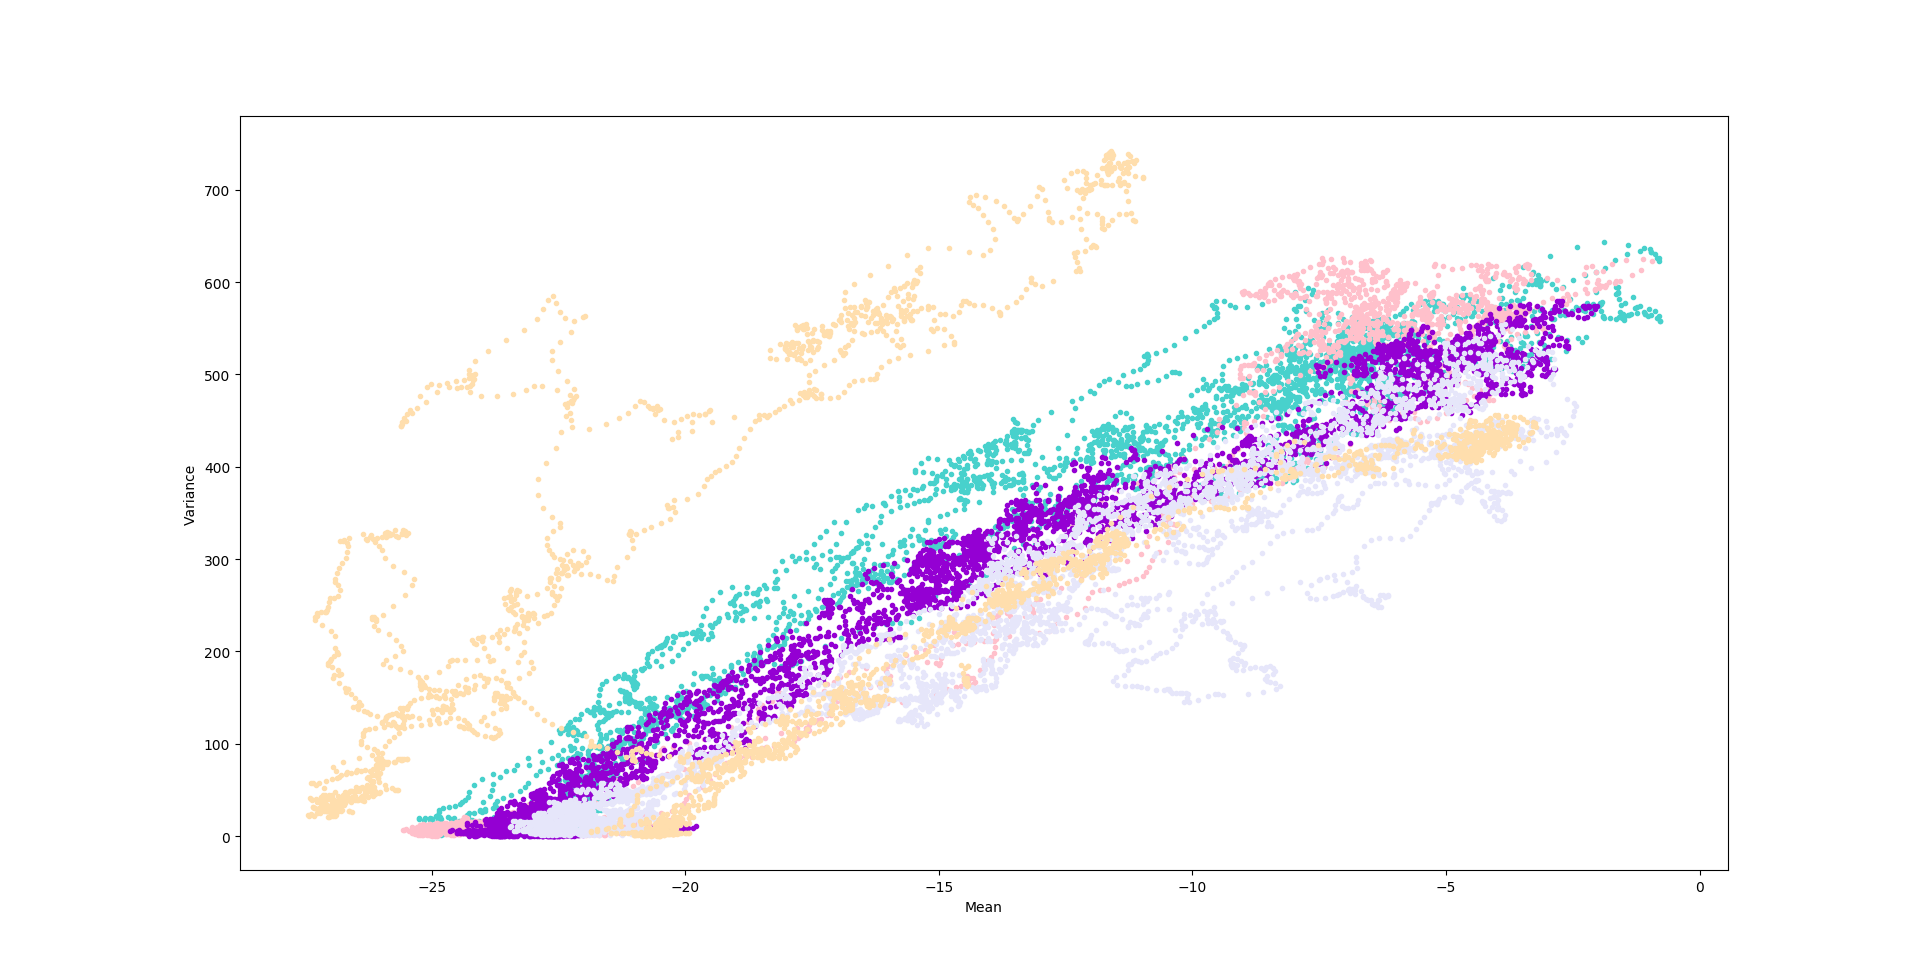
\includegraphics[width=1\linewidth]{img/plot_features}
	\caption{Grafico in 2 dimensioni della media e varianza di tutte le onde magnetiche. I colori dei punti rappresentano le etichette}
	\label{fig:plotfeatures}
\end{figure}

La causa del rumore sono i sensori che offrono una misurazione non precisa. Per risolvere, almeno in parte questo problema, \`e stato usato il \textit{filtro di Kalman} durante il preprocessamento dei dati per pulire il rumore sui dati.

\section{Codice per l'analisi dati col \textit{knn}}
\lstinputlisting[language=Python]{code/sklearn_classify.py}
Nel codice \`e stato preso come esempio il \textit{knn}, ma si puo' fare la stessa cosa con tutti gli altri classificatori. E' stata saltata la fase di pre-elaborazione dei dati perche' poco importante nel nostro caso studio mentre ci concentriamo di piu' sulla validazione degli iperparametri e la predizione di risultati per poi terminare con il calcolo dell'accuratezza. Da notare che la validazione \`e stata fatta tramite \textit{cross validation} tramite la tecnica della \textit{grid search}, che consiste semplicemente nel provare tutti i valori all'interno di \textit{$h\_params\_knn$} e selezionare quello con l'accuratezza migliore. Il paraemtro \textit{cv=5} significa che il dataset d'addestrameto \`e stato suddiviso in 5 parti. Dopo la validazione \`e stato preso il k migliore e sono stati confrontati i risultati fra un \textit{knn} con i migliori iperparametri e quelli di \textit{default}. I risultati di tale prova sono piu' avanti.


\section{Classificatori a confronto}
Qui di seguito vediamo i risultati ottenuti da ciascun classificatore con un istogramma:

\begin{figure}[H]
	\centering
	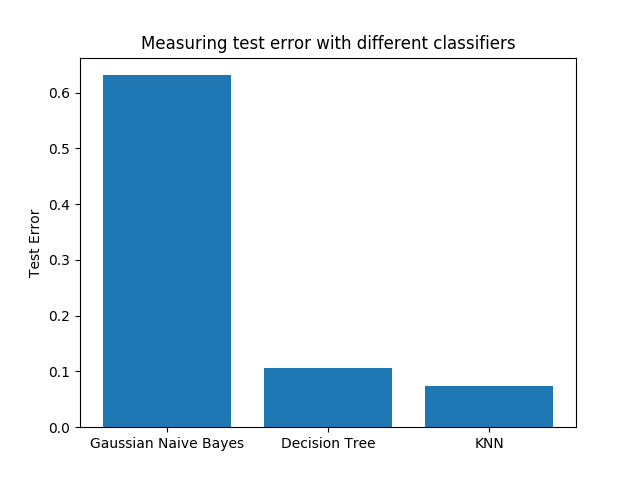
\includegraphics[width=0.7\linewidth]{img/test_errors}
	\caption{Percentuale d'errore nei test dei classificatori}
	\label{fig:testerrors}
\end{figure}

come possiamo notare \textit{Gaussian Naive Bayes} \`e totalmente inadatto alla classificazione di onde magnetiche mentre gli alberi di decisione e \textit{K Nearest Neightbours} si comportano molto bene, con risultati leggermente migliori in quest'ultimo.
A questo punto qualcuno potrebbe pero' pensare che gli ultimi 2 modelli si sono sovradattati agli esempi (\textit{overfitting}) ed avrebbe ragione, perche' applicando la \textit{cross validation} abbiamo risultati diversi da quelli precedenti.

\begin{figure}[H]
	\centering
	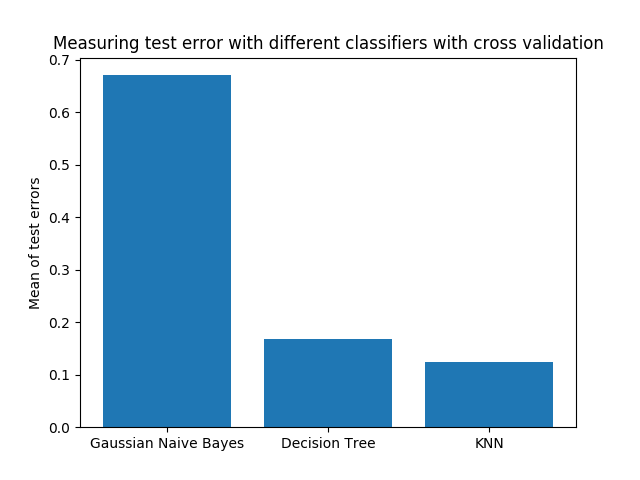
\includegraphics[width=1\linewidth]{img/test_errors_cross_validation}
	\caption{Percentuale d'errore nei test dei classificatori con la \textit{cross validation}}
	\label{fig:testerrorscrossvalidation}
\end{figure}

Adesso visualizziamo gli errori per etichetta:

\begin{figure}[H]
	\centering
	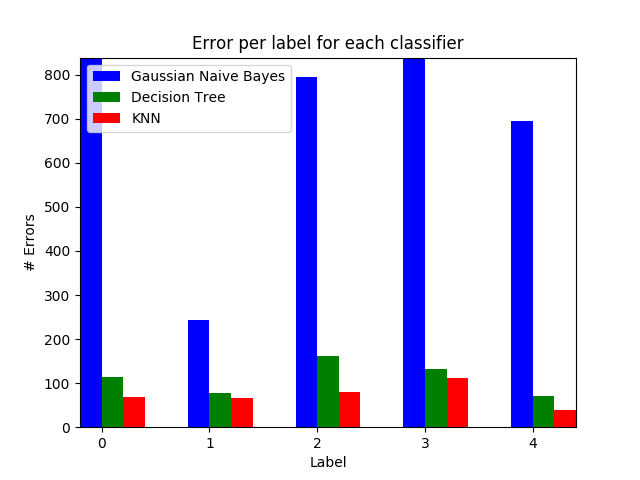
\includegraphics[width=0.7\linewidth]{img/test_error_per_label}
	\caption{Numero di errori nella predizione per etichetta}
	\label{fig:testerrorperlabel}
\end{figure}
\medskip
\begin{figure}[H]
	\centering
	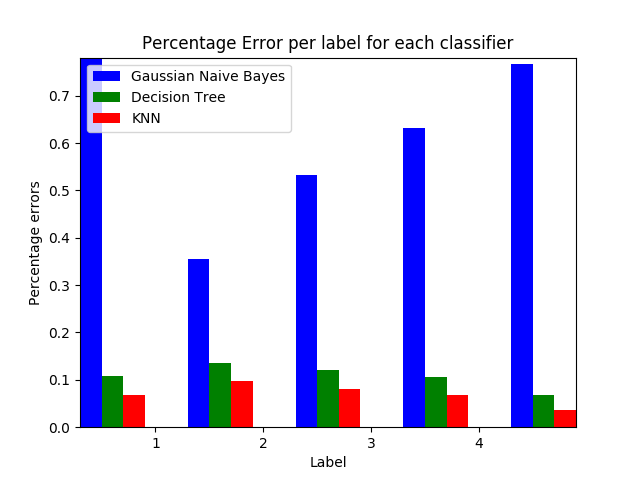
\includegraphics[width=0.7\linewidth]{img/percentage_test_errors_per_label}
	\caption{Percentuale di errore nella predizione per etichetta. Le barre blu rappresentano i risultati dei classificatori \textit{cross-validati} mentre i rossi sono quelli senza.}
	\label{fig:percentagetesterrorsperlabel}
\end{figure}

\section{Analisi del Knn al variare dell'iper parametro k}
Un grafico interessante da analizzare \`e l'accuratezza del \textit{Knn} al variare di K. L'accuratezza \`e intesa come la percentuale di predizioni azzeccate sull'insieme di test, inoltre i risultati sono stati \textit{cross validati}.
\begin{figure}[H]
	\centering
	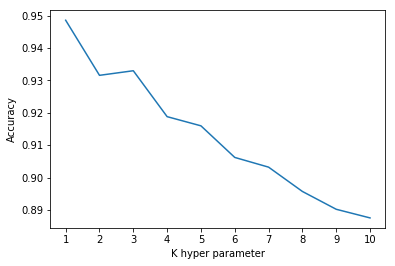
\includegraphics[width=0.7\linewidth]{img/accuracy_knn}
	\caption{Accuratezza del knn al variare di K}
	\label{fig:accuracyknn}
\end{figure}
In base a questo grafico potremmo supporre di prendere \textit{Knn} con k = 1 ma sarebbe un grave errore che porterebbe a pessimi risultati nel mondo reale. Come mai? Innanzitutto spieghiamo cio' che succede col 1-nn: per ogni nuovo punto la sua etichetta sara' quella del vicino piu' prossimo. I nostri problemi si possono ricondurre all'\textit{overfitting}, che riassumendo vuol dire che il nostro modello ha imparato troppo bene (a memoria) i nostri dati. Invece se impostiamo un k troppo alto avremo lo stesso risultato l'\textit{underfitting} ma per il motivo contrario, cioe' il nostro modello ha imparato troppo poco dai dati. Per notare veramente gli effetti dell'\textit{overfitting}, adesso vedremo su un piano cartesiano le sue conseguenze prendendo come esempio una classificazione binaria su due attributi dove ogni punto sara' colorato di blu e rosso in base alla sua etichetta. Nel grafico \`e stata tracciata una linea nera di separazione fra le due aree rosse e blu per indicare che i punti i quali andranno nell'area rossa saranno classificati come rossi dal knn e viceversa per i blu.

\begin{figure}[H]
	\centering
	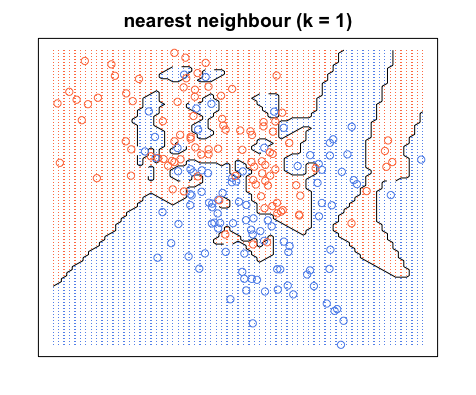
\includegraphics[width=0.7\linewidth]{img/1nearestneigh}
	\caption{Classificazione binaria con il 1-nn}
	\label{fig:1nearestneigh}
\end{figure}

\begin{figure}[H]
	\centering
	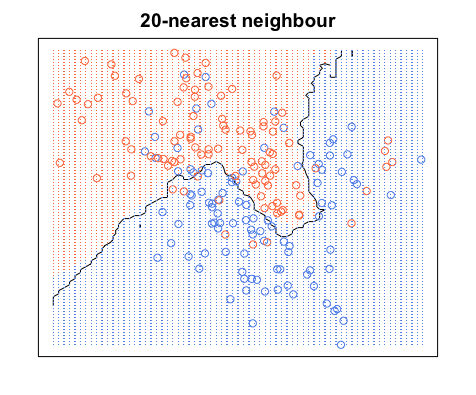
\includegraphics[width=0.7\linewidth]{img/20nearestneigh}
	\caption{Classificazione binaria con il 20-nn}
	\label{fig:20nearestneigh}
\end{figure}

Si puo' notare bene che con k=1 abbiamo sicuramente meno errori di classificazione nel nostro dataset, ma stiamo comunque ignorando il fatto che alcuni punti rossi fra i blu possono essere frutto di errore umano, sensori o di una qualsiasi fonte di dati e che quindi andrebbero ignorati. Questo risultato si ottiene andando a controllare l'etichetta di molti piu' vicini ed \`e cio' che avviene con k = 20.
Per evitare problemi di \textit{overfitting} ed \textit{underfitting} \`e necessario usare altre metriche per valutare l'efficacia del nostro modello.

\begin{figure}[H]
	\centering
	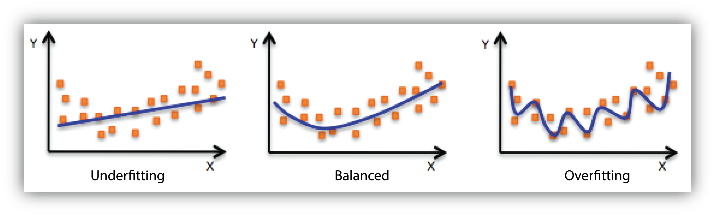
\includegraphics[width=1\linewidth]{img/underfittingoverfitting}
	\caption{\textit{Underfitting} ed \textit{overfitting} nella regressione}
	\label{fig:underfittingoverfitting}
\end{figure}

Una soluzione a questo problema \`e possibile ottenerla dalle curve di validazione che mostrano a grafico la complessita' del modello sull'asse x, quindi per esempio al variare di uno o piu' iperparamentri mentre sull'asse y l'errore sia sull'insieme di validazione che sull'insieme di addestramento.

\begin{figure}[H]
	\centering
	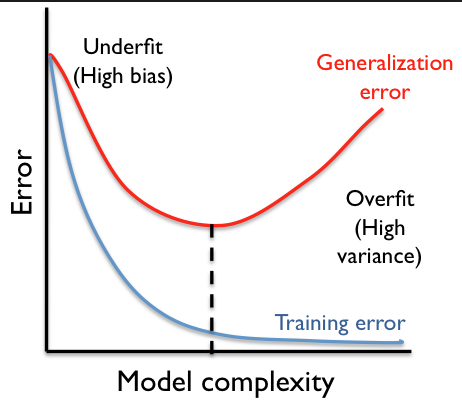
\includegraphics[width=0.7\linewidth]{img/validation_curve}
	\caption{Curve di validazione}
	\label{fig:validationcurve}
\end{figure}

Come si vede dal grafico, si dice che quando c'e' \textit{overfitting} si ha un altra varianza? Cosa vuol dire? Che stiamo modellando anche il rumore generato dai dati e cio' porta a cattive prestazioni quando ci arrivano nuove etichette da predire. Per \textit{High bias} si intente semplicemente un alto errore sulle predizioni delle etichette.
\section{Analisi del rumore durante la cattura dei dati}
Per analizzare la correttezza dei nostri dati l'approccio usato \`e stato quello di posizionarsi fermo in un punto e verificare tramite grafico che tutti i punti catturati dal magnetometro fossero concentrati in una piccola area del grafico. Purtroppo non \`e stato cosi' e ce lo dimostrano i grafici dove \`e stato messo nell'asse X il valore X catturato e sull'asse Y il valore Y.

\begin{figure}[H]
	\centering
	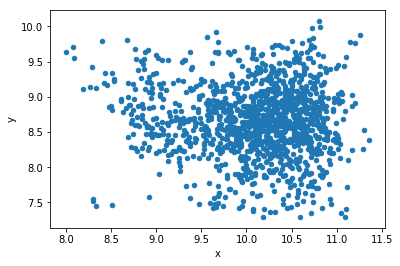
\includegraphics[width=0.7\linewidth]{img/xystand}
	\caption{Valori del magnetometro rispetto agli assi x ed y stando fermo}
	\label{fig:xystand}
\end{figure}



\section{Un rimedio ingenuo al rumore}
Un approccio ingenuo per risolvere il problema al rumore potrebbe essere quello di prendere meno dati per etichetta. Il seguente grafico pero' ci mostra che cio' non \`e vero

\begin{figure}[H]
	\centering
	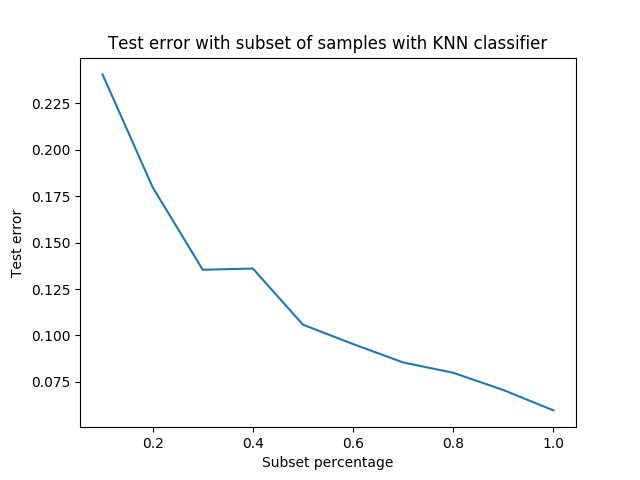
\includegraphics[width=0.7\linewidth]{img/rumor_graph_knn}
	\caption{Percentuale d'errore al variare della grandezza dell'insieme di addestramento con KNN}
	\label{fig:rumorgraphknn}
\end{figure}

Notiamo che questo grafico dimostra che all'aumentare del dataset otteniamo risultati piu' accurati poiche' ci stiamo avvicinando alla media e varianza della popolazione.

%Ricorda di far vedere falsi positivi e veri negativi nei test
\chapter{Miglioramenti}
\section{Possibili miglioramenti per la raccolta di dati}
\begin{itemize}
	\item L'architettura \textit{client-server} e' necessaria per avere un'applicazione che riesca a gestire con fluidita' la ricerca all'interno di grandi edifici. In rifermento alla memoria del telefono poiche' nella maggior parte dei casi possiede un quantitativo di \textit{RAM} e memoria permanente molto limitati, ma anche rispetto al processore perche' la ricerca della posizione, assumendo di usare il \textit{KNN}, ha bisogno di confrontare i propri attributi con tutti gli altri e va da se che piu' e' grande il dataset, piu' potenza di calcolo ci vorra' per ottenere una risposta in tempi umani.
	\item Durante la raccolta sarebbe opportuno applicare il \textit{filtro di Kalman} per ridurre il rumore causato dall'imprecisione dei sensori.
	\item Per migliorare la precisione sarebbe opportuno appoggiarsi anche ad altri sensori presenti sullo \textit{smartphone}. Prendiamo come esempio il Wi-Fi, se il dispositivo e' connesso alla rete dell'edificio potrebbe sfruttare la potenza di segnale per avere una precisione maggiore; sfruttare l'accelerometro per stimare la velocita' del telefono e quindi standardizzare tutte le rilevazioni effettuate col magnetometro. Questa tecnica viene chiamata \textit{sensor fusion}(Link a qualche paper)
\end{itemize}
%--------------------------------------------------------------
\end{document}
%--------------------------------------------------------------
\grid
